% Options for packages loaded elsewhere
\PassOptionsToPackage{unicode}{hyperref}
\PassOptionsToPackage{hyphens}{url}
\PassOptionsToPackage{dvipsnames,svgnames,x11names}{xcolor}
%
\documentclass[
  letterpaper,
  DIV=11,
  numbers=noendperiod]{scrartcl}

\usepackage{amsmath,amssymb}
\usepackage{iftex}
\ifPDFTeX
  \usepackage[T1]{fontenc}
  \usepackage[utf8]{inputenc}
  \usepackage{textcomp} % provide euro and other symbols
\else % if luatex or xetex
  \usepackage{unicode-math}
  \defaultfontfeatures{Scale=MatchLowercase}
  \defaultfontfeatures[\rmfamily]{Ligatures=TeX,Scale=1}
\fi
\usepackage{lmodern}
\ifPDFTeX\else  
    % xetex/luatex font selection
\fi
% Use upquote if available, for straight quotes in verbatim environments
\IfFileExists{upquote.sty}{\usepackage{upquote}}{}
\IfFileExists{microtype.sty}{% use microtype if available
  \usepackage[]{microtype}
  \UseMicrotypeSet[protrusion]{basicmath} % disable protrusion for tt fonts
}{}
\makeatletter
\@ifundefined{KOMAClassName}{% if non-KOMA class
  \IfFileExists{parskip.sty}{%
    \usepackage{parskip}
  }{% else
    \setlength{\parindent}{0pt}
    \setlength{\parskip}{6pt plus 2pt minus 1pt}}
}{% if KOMA class
  \KOMAoptions{parskip=half}}
\makeatother
\usepackage{xcolor}
\setlength{\emergencystretch}{3em} % prevent overfull lines
\setcounter{secnumdepth}{-\maxdimen} % remove section numbering
% Make \paragraph and \subparagraph free-standing
\makeatletter
\ifx\paragraph\undefined\else
  \let\oldparagraph\paragraph
  \renewcommand{\paragraph}{
    \@ifstar
      \xxxParagraphStar
      \xxxParagraphNoStar
  }
  \newcommand{\xxxParagraphStar}[1]{\oldparagraph*{#1}\mbox{}}
  \newcommand{\xxxParagraphNoStar}[1]{\oldparagraph{#1}\mbox{}}
\fi
\ifx\subparagraph\undefined\else
  \let\oldsubparagraph\subparagraph
  \renewcommand{\subparagraph}{
    \@ifstar
      \xxxSubParagraphStar
      \xxxSubParagraphNoStar
  }
  \newcommand{\xxxSubParagraphStar}[1]{\oldsubparagraph*{#1}\mbox{}}
  \newcommand{\xxxSubParagraphNoStar}[1]{\oldsubparagraph{#1}\mbox{}}
\fi
\makeatother

\usepackage{color}
\usepackage{fancyvrb}
\newcommand{\VerbBar}{|}
\newcommand{\VERB}{\Verb[commandchars=\\\{\}]}
\DefineVerbatimEnvironment{Highlighting}{Verbatim}{commandchars=\\\{\}}
% Add ',fontsize=\small' for more characters per line
\usepackage{framed}
\definecolor{shadecolor}{RGB}{241,243,245}
\newenvironment{Shaded}{\begin{snugshade}}{\end{snugshade}}
\newcommand{\AlertTok}[1]{\textcolor[rgb]{0.68,0.00,0.00}{#1}}
\newcommand{\AnnotationTok}[1]{\textcolor[rgb]{0.37,0.37,0.37}{#1}}
\newcommand{\AttributeTok}[1]{\textcolor[rgb]{0.40,0.45,0.13}{#1}}
\newcommand{\BaseNTok}[1]{\textcolor[rgb]{0.68,0.00,0.00}{#1}}
\newcommand{\BuiltInTok}[1]{\textcolor[rgb]{0.00,0.23,0.31}{#1}}
\newcommand{\CharTok}[1]{\textcolor[rgb]{0.13,0.47,0.30}{#1}}
\newcommand{\CommentTok}[1]{\textcolor[rgb]{0.37,0.37,0.37}{#1}}
\newcommand{\CommentVarTok}[1]{\textcolor[rgb]{0.37,0.37,0.37}{\textit{#1}}}
\newcommand{\ConstantTok}[1]{\textcolor[rgb]{0.56,0.35,0.01}{#1}}
\newcommand{\ControlFlowTok}[1]{\textcolor[rgb]{0.00,0.23,0.31}{\textbf{#1}}}
\newcommand{\DataTypeTok}[1]{\textcolor[rgb]{0.68,0.00,0.00}{#1}}
\newcommand{\DecValTok}[1]{\textcolor[rgb]{0.68,0.00,0.00}{#1}}
\newcommand{\DocumentationTok}[1]{\textcolor[rgb]{0.37,0.37,0.37}{\textit{#1}}}
\newcommand{\ErrorTok}[1]{\textcolor[rgb]{0.68,0.00,0.00}{#1}}
\newcommand{\ExtensionTok}[1]{\textcolor[rgb]{0.00,0.23,0.31}{#1}}
\newcommand{\FloatTok}[1]{\textcolor[rgb]{0.68,0.00,0.00}{#1}}
\newcommand{\FunctionTok}[1]{\textcolor[rgb]{0.28,0.35,0.67}{#1}}
\newcommand{\ImportTok}[1]{\textcolor[rgb]{0.00,0.46,0.62}{#1}}
\newcommand{\InformationTok}[1]{\textcolor[rgb]{0.37,0.37,0.37}{#1}}
\newcommand{\KeywordTok}[1]{\textcolor[rgb]{0.00,0.23,0.31}{\textbf{#1}}}
\newcommand{\NormalTok}[1]{\textcolor[rgb]{0.00,0.23,0.31}{#1}}
\newcommand{\OperatorTok}[1]{\textcolor[rgb]{0.37,0.37,0.37}{#1}}
\newcommand{\OtherTok}[1]{\textcolor[rgb]{0.00,0.23,0.31}{#1}}
\newcommand{\PreprocessorTok}[1]{\textcolor[rgb]{0.68,0.00,0.00}{#1}}
\newcommand{\RegionMarkerTok}[1]{\textcolor[rgb]{0.00,0.23,0.31}{#1}}
\newcommand{\SpecialCharTok}[1]{\textcolor[rgb]{0.37,0.37,0.37}{#1}}
\newcommand{\SpecialStringTok}[1]{\textcolor[rgb]{0.13,0.47,0.30}{#1}}
\newcommand{\StringTok}[1]{\textcolor[rgb]{0.13,0.47,0.30}{#1}}
\newcommand{\VariableTok}[1]{\textcolor[rgb]{0.07,0.07,0.07}{#1}}
\newcommand{\VerbatimStringTok}[1]{\textcolor[rgb]{0.13,0.47,0.30}{#1}}
\newcommand{\WarningTok}[1]{\textcolor[rgb]{0.37,0.37,0.37}{\textit{#1}}}

\providecommand{\tightlist}{%
  \setlength{\itemsep}{0pt}\setlength{\parskip}{0pt}}\usepackage{longtable,booktabs,array}
\usepackage{calc} % for calculating minipage widths
% Correct order of tables after \paragraph or \subparagraph
\usepackage{etoolbox}
\makeatletter
\patchcmd\longtable{\par}{\if@noskipsec\mbox{}\fi\par}{}{}
\makeatother
% Allow footnotes in longtable head/foot
\IfFileExists{footnotehyper.sty}{\usepackage{footnotehyper}}{\usepackage{footnote}}
\makesavenoteenv{longtable}
\usepackage{graphicx}
\makeatletter
\def\maxwidth{\ifdim\Gin@nat@width>\linewidth\linewidth\else\Gin@nat@width\fi}
\def\maxheight{\ifdim\Gin@nat@height>\textheight\textheight\else\Gin@nat@height\fi}
\makeatother
% Scale images if necessary, so that they will not overflow the page
% margins by default, and it is still possible to overwrite the defaults
% using explicit options in \includegraphics[width, height, ...]{}
\setkeys{Gin}{width=\maxwidth,height=\maxheight,keepaspectratio}
% Set default figure placement to htbp
\makeatletter
\def\fps@figure{htbp}
\makeatother

\KOMAoption{captions}{tableheading}
\makeatletter
\@ifpackageloaded{caption}{}{\usepackage{caption}}
\AtBeginDocument{%
\ifdefined\contentsname
  \renewcommand*\contentsname{Table of contents}
\else
  \newcommand\contentsname{Table of contents}
\fi
\ifdefined\listfigurename
  \renewcommand*\listfigurename{List of Figures}
\else
  \newcommand\listfigurename{List of Figures}
\fi
\ifdefined\listtablename
  \renewcommand*\listtablename{List of Tables}
\else
  \newcommand\listtablename{List of Tables}
\fi
\ifdefined\figurename
  \renewcommand*\figurename{Figure}
\else
  \newcommand\figurename{Figure}
\fi
\ifdefined\tablename
  \renewcommand*\tablename{Table}
\else
  \newcommand\tablename{Table}
\fi
}
\@ifpackageloaded{float}{}{\usepackage{float}}
\floatstyle{ruled}
\@ifundefined{c@chapter}{\newfloat{codelisting}{h}{lop}}{\newfloat{codelisting}{h}{lop}[chapter]}
\floatname{codelisting}{Listing}
\newcommand*\listoflistings{\listof{codelisting}{List of Listings}}
\makeatother
\makeatletter
\makeatother
\makeatletter
\@ifpackageloaded{caption}{}{\usepackage{caption}}
\@ifpackageloaded{subcaption}{}{\usepackage{subcaption}}
\makeatother

\ifLuaTeX
  \usepackage{selnolig}  % disable illegal ligatures
\fi
\usepackage{bookmark}

\IfFileExists{xurl.sty}{\usepackage{xurl}}{} % add URL line breaks if available
\urlstyle{same} % disable monospaced font for URLs
\hypersetup{
  pdftitle={Lab 6},
  pdfauthor={Jazmin Hernandez},
  colorlinks=true,
  linkcolor={blue},
  filecolor={Maroon},
  citecolor={Blue},
  urlcolor={Blue},
  pdfcreator={LaTeX via pandoc}}


\title{Lab 6}
\author{Jazmin Hernandez}
\date{}

\begin{document}
\maketitle


\subsection{Lab 06 - Text Mining}\label{lab-06---text-mining}

\begin{Shaded}
\begin{Highlighting}[]
\FunctionTok{library}\NormalTok{(dplyr)}
\end{Highlighting}
\end{Shaded}

\begin{verbatim}

Attaching package: 'dplyr'
\end{verbatim}

\begin{verbatim}
The following objects are masked from 'package:stats':

    filter, lag
\end{verbatim}

\begin{verbatim}
The following objects are masked from 'package:base':

    intersect, setdiff, setequal, union
\end{verbatim}

\begin{Shaded}
\begin{Highlighting}[]
\FunctionTok{library}\NormalTok{(ggplot2)}
\FunctionTok{library}\NormalTok{(tidytext)}
\FunctionTok{library}\NormalTok{(readr)}
\NormalTok{mt\_samples }\OtherTok{\textless{}{-}} \FunctionTok{read\_csv}\NormalTok{(}\StringTok{"https://raw.githubusercontent.com/USCbiostats/data{-}science{-}data/master/00\_mtsamples/mtsamples.csv"}\NormalTok{)}
\end{Highlighting}
\end{Shaded}

\begin{verbatim}
New names:
* `` -> `...1`
\end{verbatim}

\begin{verbatim}
Rows: 4999 Columns: 6
-- Column specification --------------------------------------------------------
Delimiter: ","
chr (5): description, medical_specialty, sample_name, transcription, keywords
dbl (1): ...1

i Use `spec()` to retrieve the full column specification for this data.
i Specify the column types or set `show_col_types = FALSE` to quiet this message.
\end{verbatim}

\begin{Shaded}
\begin{Highlighting}[]
\NormalTok{mt\_samples }\OtherTok{\textless{}{-}}\NormalTok{ mt\_samples }\SpecialCharTok{|\textgreater{}}
  \FunctionTok{select}\NormalTok{(description, medical\_specialty, transcription)}

\FunctionTok{head}\NormalTok{(mt\_samples)}
\end{Highlighting}
\end{Shaded}

\begin{verbatim}
# A tibble: 6 x 3
  description                                    medical_specialty transcription
  <chr>                                          <chr>             <chr>        
1 A 23-year-old white female presents with comp~ Allergy / Immuno~ "SUBJECTIVE:~
2 Consult for laparoscopic gastric bypass.       Bariatrics        "PAST MEDICA~
3 Consult for laparoscopic gastric bypass.       Bariatrics        "HISTORY OF ~
4 2-D M-Mode. Doppler.                           Cardiovascular /~ "2-D M-MODE:~
5 2-D Echocardiogram                             Cardiovascular /~ "1.  The lef~
6 Morbid obesity.  Laparoscopic antecolic anteg~ Bariatrics        "PREOPERATIV~
\end{verbatim}

\subsubsection{Question 1}\label{question-1}

There are 40 different medical specialties. Specialties such as Cosmetic
/ Plastic Surgery and Dentistry both have 27 counts. Diets and Nutrition
and Rheumatology specialties both have counts of 10. Autopsy and Lab
Medicine - Pathology specialties both have counts of 8. There does not
appear to be an even distribution between the medical specialties as we
can see that Surgery has 1103 counts compared to\\
Hospice - Palliative Care with only 6 counts.

\begin{Shaded}
\begin{Highlighting}[]
\NormalTok{med\_specialty\_counts }\OtherTok{\textless{}{-}}\NormalTok{ mt\_samples }\SpecialCharTok{|\textgreater{}}
  \FunctionTok{count}\NormalTok{(medical\_specialty, }\AttributeTok{name =} \StringTok{"n"}\NormalTok{, }\AttributeTok{sort =} \ConstantTok{TRUE}\NormalTok{)}
\FunctionTok{print}\NormalTok{(med\_specialty\_counts)}
\end{Highlighting}
\end{Shaded}

\begin{verbatim}
# A tibble: 40 x 2
   medical_specialty                 n
   <chr>                         <int>
 1 Surgery                        1103
 2 Consult - History and Phy.      516
 3 Cardiovascular / Pulmonary      372
 4 Orthopedic                      355
 5 Radiology                       273
 6 General Medicine                259
 7 Gastroenterology                230
 8 Neurology                       223
 9 SOAP / Chart / Progress Notes   166
10 Obstetrics / Gynecology         160
# i 30 more rows
\end{verbatim}

\begin{Shaded}
\begin{Highlighting}[]
\NormalTok{overlap\_counts }\OtherTok{\textless{}{-}}\NormalTok{ mt\_samples }\SpecialCharTok{|\textgreater{}}
\FunctionTok{rowwise}\NormalTok{() }\SpecialCharTok{|\textgreater{}}
\FunctionTok{mutate}\NormalTok{(}\AttributeTok{num\_specialties =} \FunctionTok{sum}\NormalTok{(}\FunctionTok{c\_across}\NormalTok{(}\FunctionTok{starts\_with}\NormalTok{(}\StringTok{"specialty\_"}\NormalTok{)), }\AttributeTok{na.rm =} \ConstantTok{TRUE}\NormalTok{)) }\SpecialCharTok{|\textgreater{}}
\FunctionTok{count}\NormalTok{(num\_specialties)}

\FunctionTok{print}\NormalTok{(overlap\_counts)}
\end{Highlighting}
\end{Shaded}

\begin{verbatim}
# A tibble: 1 x 2
# Rowwise: 
  num_specialties     n
            <int> <int>
1               0  4999
\end{verbatim}

\subsubsection{Question 2}\label{question-2}

The list shows that the word ``the'' appears the most (149888 times) in
the text. This makes sense because stop words usually appear the most in
English text. Looking at the top tenth word that appears the most,
patient, which appears 22065 times, it does give us an insight that the
text is focused on medical transcripts mainly revolving around patient
interactions.

\begin{Shaded}
\begin{Highlighting}[]
\NormalTok{mt\_samples }\SpecialCharTok{|\textgreater{}} 
  \FunctionTok{unnest\_tokens}\NormalTok{(token, transcription) }\SpecialCharTok{|\textgreater{}} 
  \FunctionTok{count}\NormalTok{(token) }\SpecialCharTok{|\textgreater{}} 
  \FunctionTok{top\_n}\NormalTok{(}\DecValTok{20}\NormalTok{, n) }\SpecialCharTok{|\textgreater{}} 
  \FunctionTok{ggplot}\NormalTok{(}\FunctionTok{aes}\NormalTok{(n, token)) }\SpecialCharTok{+}
  \FunctionTok{geom\_col}\NormalTok{()}
\end{Highlighting}
\end{Shaded}

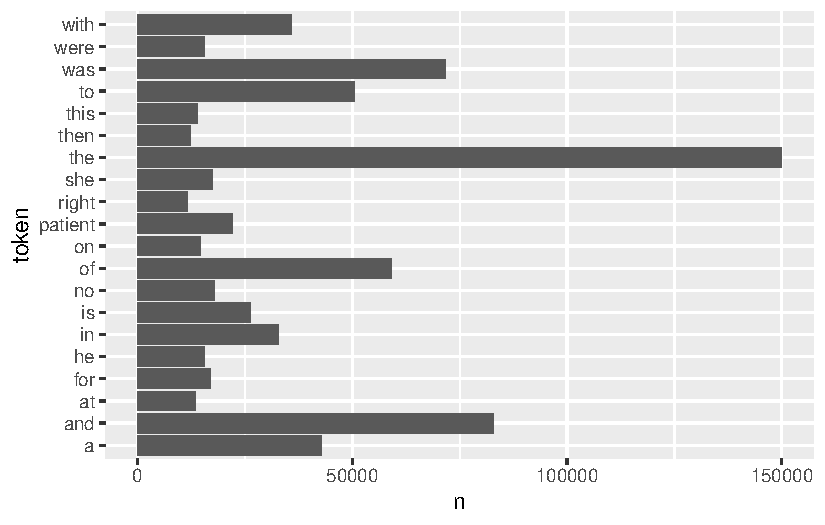
\includegraphics{Lab-6_files/figure-pdf/unnamed-chunk-3-1.pdf}

\subsubsection{Question 3}\label{question-3}

Now that we have removed stop words, we can see that the word `patient'
appears the most which is more fitting given that this is a medical
transcript. Looking at the rest of the top 20 words, it is clear that
this text is about patient procedures or charting.

\begin{Shaded}
\begin{Highlighting}[]
\FunctionTok{library}\NormalTok{(forcats)}
\FunctionTok{library}\NormalTok{(tidytext)}
\NormalTok{mt\_samples }\SpecialCharTok{|\textgreater{}} 
  \FunctionTok{unnest\_tokens}\NormalTok{(word, transcription) }\SpecialCharTok{|\textgreater{}}           
  \FunctionTok{anti\_join}\NormalTok{(stop\_words, }\AttributeTok{by =} \StringTok{"word"}\NormalTok{) }\SpecialCharTok{|\textgreater{}}             
  \FunctionTok{filter}\NormalTok{(}\SpecialCharTok{!}\FunctionTok{grepl}\NormalTok{(}\StringTok{"[0{-}9]"}\NormalTok{, word)) }\SpecialCharTok{|\textgreater{}}                   
  \FunctionTok{count}\NormalTok{(word, }\AttributeTok{sort =} \ConstantTok{TRUE}\NormalTok{) }\SpecialCharTok{|\textgreater{}}                        
  \FunctionTok{top\_n}\NormalTok{(}\DecValTok{20}\NormalTok{, n) }\SpecialCharTok{|\textgreater{}}                                    
  \FunctionTok{ggplot}\NormalTok{(}\FunctionTok{aes}\NormalTok{(n, }\FunctionTok{fct\_reorder}\NormalTok{(word, n))) }\SpecialCharTok{+}
  \FunctionTok{geom\_col}\NormalTok{()}
\end{Highlighting}
\end{Shaded}

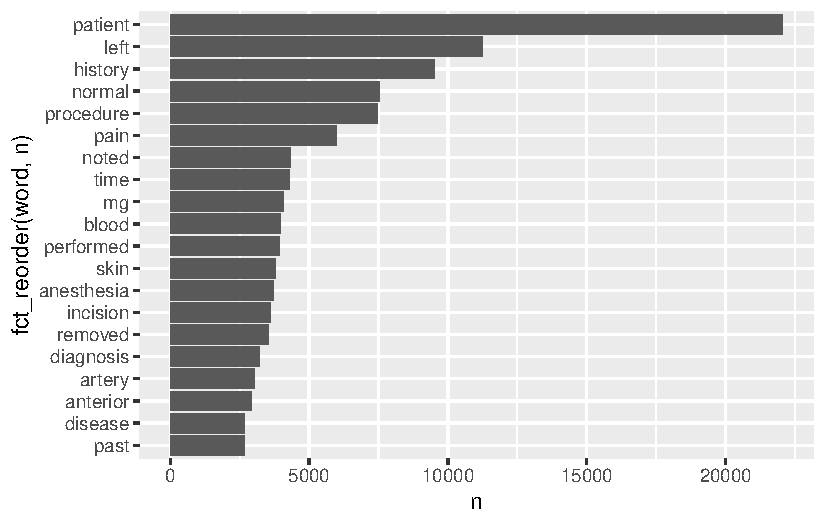
\includegraphics{Lab-6_files/figure-pdf/unnamed-chunk-4-1.pdf}

\subsubsection{Question 4}\label{question-4}

We have a lot more insight into what the text is about when tokenizing
into tri-grams rather than bi-grams. Bi-grams is mostly stop words but
looking at tri-grams, we can see more insight into procedures and even
patient symptoms.

\begin{Shaded}
\begin{Highlighting}[]
\NormalTok{mt\_samples }\SpecialCharTok{|\textgreater{}} 
\FunctionTok{unnest\_tokens}\NormalTok{(bigram, transcription, }\AttributeTok{token =} \StringTok{"ngrams"}\NormalTok{, }\AttributeTok{n =} \DecValTok{2}\NormalTok{) }\SpecialCharTok{|\textgreater{}}
\FunctionTok{count}\NormalTok{(bigram, }\AttributeTok{sort =} \ConstantTok{TRUE}\NormalTok{)}
\end{Highlighting}
\end{Shaded}

\begin{verbatim}
# A tibble: 301,415 x 2
   bigram          n
   <chr>       <int>
 1 the patient 20307
 2 of the      19062
 3 in the      12790
 4 to the      12374
 5 was then     6956
 6 and the      6350
 7 patient was  6293
 8 the right    5509
 9 on the       5241
10 the left     4860
# i 301,405 more rows
\end{verbatim}

\begin{Shaded}
\begin{Highlighting}[]
\NormalTok{mt\_samples }\SpecialCharTok{|\textgreater{}}
  \FunctionTok{unnest\_tokens}\NormalTok{(trigram, transcription, }\AttributeTok{token =} \StringTok{"ngrams"}\NormalTok{, }\AttributeTok{n =} \DecValTok{3}\NormalTok{) }\SpecialCharTok{|\textgreater{}}
  \FunctionTok{count}\NormalTok{(trigram, }\AttributeTok{sort =} \ConstantTok{TRUE}\NormalTok{)}
\end{Highlighting}
\end{Shaded}

\begin{verbatim}
# A tibble: 655,441 x 2
   trigram                n
   <chr>              <int>
 1 the patient was     6104
 2 the patient is      3075
 3 as well as          2243
 4 there is no         1678
 5 the operating room  1532
 6 patient is a        1491
 7 prepped and draped  1490
 8 was used to         1480
 9 and draped in       1372
10 at this time        1333
# i 655,431 more rows
\end{verbatim}

\subsubsection{Question 5}\label{question-5}

\begin{Shaded}
\begin{Highlighting}[]
\FunctionTok{library}\NormalTok{(stringr)}
\FunctionTok{library}\NormalTok{(tidyr)}
\NormalTok{word\_to\_analyze }\OtherTok{\textless{}{-}} \StringTok{"patient"}
\NormalTok{bi\_grams }\OtherTok{\textless{}{-}}\NormalTok{ mt\_samples}\SpecialCharTok{|\textgreater{}}
\FunctionTok{unnest\_tokens}\NormalTok{(bigram, transcription, }\AttributeTok{token =} \StringTok{"ngrams"}\NormalTok{, }\AttributeTok{n =} \DecValTok{2}\NormalTok{) }
\FunctionTok{print}\NormalTok{(}\FunctionTok{head}\NormalTok{(bi\_grams))}
\end{Highlighting}
\end{Shaded}

\begin{verbatim}
# A tibble: 6 x 3
  description                                           medical_specialty bigram
  <chr>                                                 <chr>             <chr> 
1 A 23-year-old white female presents with complaint o~ Allergy / Immuno~ subje~
2 A 23-year-old white female presents with complaint o~ Allergy / Immuno~ this ~
3 A 23-year-old white female presents with complaint o~ Allergy / Immuno~ 23 ye~
4 A 23-year-old white female presents with complaint o~ Allergy / Immuno~ year ~
5 A 23-year-old white female presents with complaint o~ Allergy / Immuno~ old w~
6 A 23-year-old white female presents with complaint o~ Allergy / Immuno~ white~
\end{verbatim}

\begin{Shaded}
\begin{Highlighting}[]
\NormalTok{before\_after }\OtherTok{\textless{}{-}}\NormalTok{ bi\_grams}\SpecialCharTok{|\textgreater{}}
\FunctionTok{filter}\NormalTok{(}\FunctionTok{str\_detect}\NormalTok{(bigram, word\_to\_analyze))}
\NormalTok{before\_after }\OtherTok{\textless{}{-}}\NormalTok{ before\_after }\SpecialCharTok{|\textgreater{}}
\FunctionTok{separate}\NormalTok{(bigram, }\AttributeTok{into =} \FunctionTok{c}\NormalTok{(}\StringTok{"word1"}\NormalTok{, }\StringTok{"word2"}\NormalTok{), }\AttributeTok{sep =} \StringTok{" "}\NormalTok{)}
\end{Highlighting}
\end{Shaded}

\begin{Shaded}
\begin{Highlighting}[]
\NormalTok{before\_count }\OtherTok{\textless{}{-}}\NormalTok{ before\_after }\SpecialCharTok{|\textgreater{}}
\FunctionTok{filter}\NormalTok{(word2 }\SpecialCharTok{==}\NormalTok{ word\_to\_analyze) }\SpecialCharTok{|\textgreater{}}
\FunctionTok{count}\NormalTok{(word1, }\AttributeTok{sort =} \ConstantTok{TRUE}\NormalTok{) }\SpecialCharTok{|\textgreater{}}
\FunctionTok{rename}\NormalTok{(}\AttributeTok{before =}\NormalTok{ word1)}

\NormalTok{after\_count }\OtherTok{\textless{}{-}}\NormalTok{ before\_after }\SpecialCharTok{|\textgreater{}}
\FunctionTok{filter}\NormalTok{(word1 }\SpecialCharTok{==}\NormalTok{ word\_to\_analyze) }\SpecialCharTok{|\textgreater{}}
\FunctionTok{count}\NormalTok{(word2, }\AttributeTok{sort =} \ConstantTok{TRUE}\NormalTok{) }\SpecialCharTok{|\textgreater{}}
\FunctionTok{rename}\NormalTok{(}\AttributeTok{after =}\NormalTok{ word2)}
\end{Highlighting}
\end{Shaded}

\begin{Shaded}
\begin{Highlighting}[]
\FunctionTok{print}\NormalTok{(}\StringTok{"Words Before \textquotesingle{}patient\textquotesingle{}:"}\NormalTok{)}
\end{Highlighting}
\end{Shaded}

\begin{verbatim}
[1] "Words Before 'patient':"
\end{verbatim}

\begin{Shaded}
\begin{Highlighting}[]
\FunctionTok{print}\NormalTok{(before\_count)}
\end{Highlighting}
\end{Shaded}

\begin{verbatim}
# A tibble: 269 x 2
   before        n
   <chr>     <int>
 1 the       20307
 2 this        470
 3 history     101
 4 a            67
 5 and          47
 6 procedure    32
 7 female       26
 8 with         25
 9 use          24
10 old          23
# i 259 more rows
\end{verbatim}

\begin{Shaded}
\begin{Highlighting}[]
\FunctionTok{print}\NormalTok{(}\StringTok{"Words After \textquotesingle{}patient\textquotesingle{}:"}\NormalTok{)}
\end{Highlighting}
\end{Shaded}

\begin{verbatim}
[1] "Words After 'patient':"
\end{verbatim}

\begin{Shaded}
\begin{Highlighting}[]
\FunctionTok{print}\NormalTok{(after\_count)}
\end{Highlighting}
\end{Shaded}

\begin{verbatim}
# A tibble: 588 x 2
   after         n
   <chr>     <int>
 1 was        6293
 2 is         3332
 3 has        1417
 4 tolerated   994
 5 had         888
 6 will        616
 7 denies      552
 8 and         377
 9 states      363
10 does        334
# i 578 more rows
\end{verbatim}

\subsubsection{Question 6}\label{question-6}

The most used word in allergy/immunology is `history.' Autopsy is
`left,' Bariatrics is `patient,' etc. The top 5 most used words include
`patient' `left' `history' `2', and `1'.

\begin{Shaded}
\begin{Highlighting}[]
\NormalTok{most\_used\_words }\OtherTok{\textless{}{-}}\NormalTok{ mt\_samples }\SpecialCharTok{|\textgreater{}}
  \FunctionTok{unnest\_tokens}\NormalTok{(word, transcription) }\SpecialCharTok{|\textgreater{}}
  \FunctionTok{anti\_join}\NormalTok{(stop\_words, }\AttributeTok{by =} \StringTok{"word"}\NormalTok{) }\SpecialCharTok{|\textgreater{}}
  \FunctionTok{group\_by}\NormalTok{(medical\_specialty, word) }\SpecialCharTok{|\textgreater{}}
  \FunctionTok{count}\NormalTok{(}\AttributeTok{n =} \FunctionTok{n}\NormalTok{(), }\AttributeTok{sort =} \ConstantTok{TRUE}\NormalTok{) }\SpecialCharTok{|\textgreater{}}
  \FunctionTok{arrange}\NormalTok{(medical\_specialty, }\FunctionTok{desc}\NormalTok{(n))   }
\end{Highlighting}
\end{Shaded}

\begin{verbatim}
Storing counts in `nn`, as `n` already present in input
i Use `name = "new_name"` to pick a new name.
\end{verbatim}

\begin{Shaded}
\begin{Highlighting}[]
\FunctionTok{print}\NormalTok{ (most\_used\_words)}
\end{Highlighting}
\end{Shaded}

\begin{verbatim}
# A tibble: 149,973 x 4
# Groups:   medical_specialty, word [149,973]
   medical_specialty    word              n    nn
   <chr>                <chr>         <int> <int>
 1 Allergy / Immunology history     1263045    38
 2 Allergy / Immunology noted       1263045    23
 3 Allergy / Immunology patient     1263045    22
 4 Allergy / Immunology allergies   1263045    21
 5 Allergy / Immunology nasal       1263045    13
 6 Allergy / Immunology past        1263045    13
 7 Allergy / Immunology bilaterally 1263045    12
 8 Allergy / Immunology masses      1263045    12
 9 Allergy / Immunology asthma      1263045    11
10 Allergy / Immunology medical     1263045    11
# i 149,963 more rows
\end{verbatim}

\begin{Shaded}
\begin{Highlighting}[]
\NormalTok{most\_used\_words }\OtherTok{\textless{}{-}}\NormalTok{ mt\_samples}\SpecialCharTok{|\textgreater{}}
  \FunctionTok{unnest\_tokens}\NormalTok{(word, transcription)}\SpecialCharTok{|\textgreater{}}      
  \FunctionTok{anti\_join}\NormalTok{(stop\_words, }\AttributeTok{by =} \StringTok{"word"}\NormalTok{) }\SpecialCharTok{|\textgreater{}}        
  \FunctionTok{count}\NormalTok{(word, }\AttributeTok{sort =} \ConstantTok{TRUE}\NormalTok{) }\SpecialCharTok{|\textgreater{}}               
  \FunctionTok{top\_n}\NormalTok{(}\DecValTok{5}\NormalTok{, n)}
\FunctionTok{print}\NormalTok{(most\_used\_words)}
\end{Highlighting}
\end{Shaded}

\begin{verbatim}
# A tibble: 5 x 2
  word        n
  <chr>   <int>
1 patient 22065
2 left    11258
3 history  9509
4 2        8864
5 1        8396
\end{verbatim}




\end{document}
